\documentclass[10pt]{beamer}
% \documentclass[handout,10pt]{beamer}
\usepackage{my_style}
%%%%%%%%%%%%%%%%%%%%%%%%%%%%%%%%%%%%%%%%%%%%%%%%%%%%%%%%%%%%%%%%%%%%%%%%

\title[Math/CS 375]{Lecture 11 - A}
\subtitle{\S 5.1, 5.3 Numerical Integration}


\begin{document}
\begin{frame}
  \titlepage
\end{frame}
%%%%%%%%%%%%%%%%%%%%%%%%%%%%%%%%%%%%%%%%%%%
\begin{frame}{Goals}
We will answer these questions:\\[3mm]
\begin{itemize}
    \item What is numerical integration and why do we care?
    \item What are Riemann sums and how are they insufficient for numerical integration?
    \item What is the trapezoidal method and how accurate is it?
    \item What is Simpson's rule and how accurate is it?
    \item What are Newton-Cotes rules and how are they related to splines? 
\end{itemize}
\end{frame}
%%%%%%%%%%%%%%%%%%%%%%%%%%%%%%%%%%%%%%%%%%%
\sectionframe{Why Numerical Integration?}
%%%%%%%%%%%%%%%%%%%%%%%%%%%%%%%%%%%%%%%%%%%
\begin{frame}{What is Numerical Integration?}
    \define{Numerical Integration}{
    \textbf{Numerical integration} refers to a method which approximates the integral $$\int_\Omega f(X)\,dX.$$
    }
    \begin{itemize}
        \item For this class, we will only cover 1D integrals 
            $$\int_a^b f(x)\,dx$$
        \item All 1D numerical integration discussed do carry over to higher dimensions
    \end{itemize}
\end{frame}

%%%%%%%%%%%%%%%%%%%%%%%%%%%%%%%%%%%%%%%%%%%
\begin{frame}[shrink]{Motivation for Numerical Integration}
\begin{itemize}
    \item Suppose you observe data points $(x_i,y_i)$ that come from an unknown function $$y=f(x)$$
        \begin{center}
            
        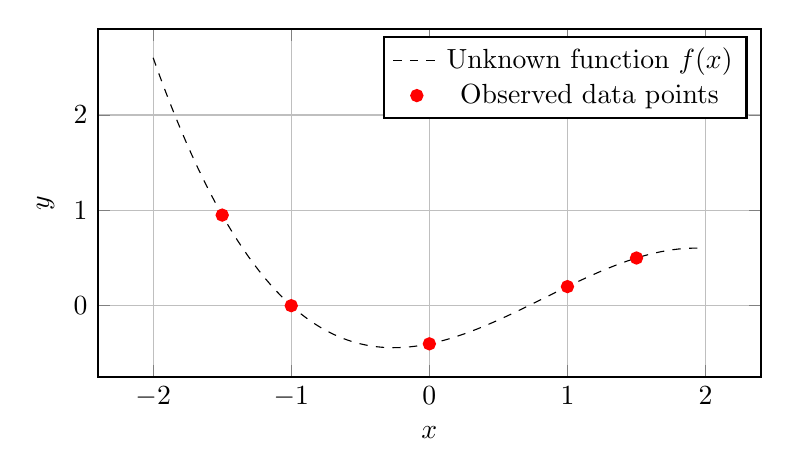
\begin{tikzpicture}
        \begin{axis}[
        width=10cm, height=6cm,
        xlabel={$x$}, ylabel={$y$},
        grid=major, 
        thick,
        domain=-2:2,
        samples=100,
        % legend pos=outer south
        ]
        % Polynomial interpolation curve
        \addplot[color=black, thin, dashed] {-0.2*x^3 + 0.5*x^2 + 0.3*x - 0.4};
        
        % Interpolation points
        \addplot[color=red, only marks, mark=*] 
        coordinates { (-1.5,0.95) (-1, 0) (0, -0.4) (1, 0.2) (1.5, 0.5)};
        
        % Optional legend
        \legend{Unknown function $f(x)$, Observed data points};
        \end{axis}
        \end{tikzpicture}
        \end{center}
        
    \item We can approximate the integral
        \begin{equation*}
          \int_{a}^{b} f(x) \,dx
        \end{equation*}
        even when $f(x)$ is unknown
\end{itemize}
\end{frame}

%%%%%%%%%%%%%%%%%%%%%%%%%%%%%%%%%%%%%%%%%%%
\begin{frame}[shrink]{Motivation for Numerical Integration}
\begin{itemize}
    \item Suppose you \emph{did} know $f(x)$ but you had no way of finding the antiderivative 
        \begin{center}
        
        \begin{tikzpicture}
        \begin{axis}[
            width=10cm, height=6cm,
            xlabel={$x$}, ylabel={$y$},
            grid=major, 
            thick,
            domain=-2:2,
            samples=100,
        ]
        
            % Define the curve
            \addplot[name path=f, color=black, thin] {exp(-x^2)};
        
            % Define the x-axis as a path
            \path[name path=axis] (\pgfkeysvalueof{/pgfplots/xmin},0) -- (\pgfkeysvalueof{/pgfplots/xmax},0);
        
            % Define the clipping path for shading
            \def\clippath{
                (-1,0) rectangle (1,1)
            }
        
            % Draw the curve with shading
            \addplot +[
                name path=A, domain=-1:1, 
                mark=none,
                postaction={decorate, red, line width=1pt, 
                    decoration={ 
                        soft clip,
                        soft clip path={\clippath},
                    },
                },
            ] {exp(-x^2)};
        
            % Shade the area between the curve and the x-axis
            \addplot [blue, fill=blue!80, fill opacity=0.2]
            fill between [
                of=A and axis,
                soft clip={domain=-1:1},
            ];
        
            % Optional legend
            \legend{$f(x) = e^{-x^2}$};
        \end{axis}
        \end{tikzpicture}
        \end{center}
        
    \item We can approximate the value of
        \begin{equation*}
          \int_{a}^{b} f(x) \,dx
        \end{equation*}
        even when the anti-derivative does not exist in closed form.
\end{itemize}
\end{frame}
%%%%%%%%%%%%%%%%%%%%%%%%%%%%%%%%%%%%%%%%%%%
\begin{frame}{More Examples}
There are many more examples:
\begin{itemize}
    \item $\int e^{-x^3}\,dx$
    \item $\int \sin(x^2)\,dx$
    \item $\int e^{\sin x}\,dx$
    \item $\int \sqrt{1+x^3}\,dx$
    \item $\int \frac{\tan x}{x}\,dx$
    \item $\int \ln\ln x\,dx$
    \item $\int x^x\,dx$
\end{itemize}
    \keyidea{There's no closed-form solution but we still want to evaluate them.}
\end{frame}
%%%%%%%%%%%%%%%%%%%%%%%%%%%%%%%%%%%%%%%%%%%
\begin{frame}{Why?}
Integrals have meaningful information:\\[2mm]
\begin{itemize}
    \item Total distance traveled 
    \item Total work done 
    \item Total mass 
    \item Center of mass
    \item Total revenue
    \item Total anything\\ $\vdots$
    \item Differential equations 
\end{itemize}
\end{frame}
%%%%%%%%%%%%%%%%%%%%%%%%%%%%%%%%%%%%%%%%%%%
\sectionframe{What is a Riemann Sum?}
%%%%%%%%%%%%%%%%%%%%%%%%%%%%%%%%%%%%%%%%%%%
\begin{frame}[shrink]{Riemann Sums}{Definitions}
\define{Partition}{
\begin{itemize}
    \item The \textbf{partition} of $[a,b]$ is a set of $n+1$ distinct and ordered points 
        $$P=\{x_0=a,\; x_1,\, x_2,\, \ldots,x_i,\, x_{i+1},\, \ldots \;, x_n =b\}$$ 
    \item The \textbf{subinterval} $[x_i, x_{i+1}]$ has a width of $\Delta x_i = x_{i+1}-x_i$. 

    \item The \textbf{sample point} $x_i^* \in [x_i, x_{i+1}]$ acts as a representative of the subinterval. 
\end{itemize}
}

\define{Riemann Sum}{
\begin{itemize}
  \item Let $y=f(x)$ be defined over $[a,b]$ that is divided into a partition $P$.
  \item Then the \textbf{Riemann sum} of $f(x)$ over the partition $P$ is defined to be 
    $$R(f,P) = \sum_{i=0}^{n-1} f(x^*_i) \Delta x_i $$

\end{itemize}
}
\end{frame}
%%%%%%%%%%%%%%%%%%%%%%%%%%%%%%%%%%%%%%%%%%%

\begin{frame}{Upper and Lower Riemann Sums}
\define{Upper and Lower Sums}{
\begin{itemize}
    \item Let $m_i $ be the \textbf{lower bound} of $f$ on $[x_i,x_{i+1}]$
    \item Let $M_i$ be the \textbf{upper bound} of $f$ on $[x_i,x_{i+1}]$ 
    \item The \textbf{Lower Sum} of $f$ on $P$ is
        \begin{equation*}
        L(f;P) = \sum_{i=0}^{n-1} m_i \Delta x_i
        \end{equation*}
    \item The \textbf{Upper Sum} of $f$ on $P$ is
        \begin{equation*}
        U(f;P) = \sum_{i=0}^{n-1} M_i \Delta x_i
        \end{equation*}
\end{itemize}
}

These are tools to define the integral
$$
I = \int_a^b f(x)\,dx
$$

\end{frame}

%%%%%%%%%%%%%%%%%%%%%%%%%%%%%%%%%%%%%%%%%%%
\begin{frame}{Graphically: Integral}
\begin{center}
  % 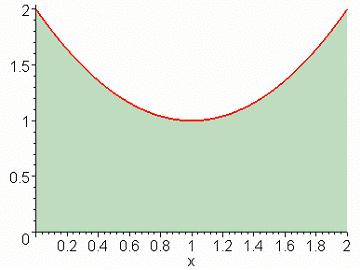
\includegraphics[height=6cm]{./figs/integral}
\begin{tikzpicture}
\begin{axis}[
    width=10cm, height=6cm,
    xlabel={$x$}, ylabel={},
    domain=0:2,
    samples=200,
    axis lines=left,
    xtick={0,0.4,0.8,1.2,1.6,2},
    ytick={0,0.5,1,1.5,2},
    ticklabel style={font=\small},
    enlargelimits=false,
    clip=false,
    grid=none,
    ymin=0, ymax=2.2,
    xmin=0, xmax=2,
    axis on top,
]

% Function
\addplot [
    name path=f,
    domain=0:2,
    red,
    thick
] { (x - 1)^2+1};

% x-axis path
\path[name path=axis] (axis cs:0,0) -- (axis cs:2,0);

% Fill area under the curve
\addplot [
    fill=blue!30,
    fill opacity=0.6,
    draw=none
] fill between[
    of=f and axis,
];
\end{axis}
\end{tikzpicture}

The area of the shaded region is what we want to calculate
$$
    I=\int_0^2 f(x)\,dx
$$
\end{center}
\end{frame}

%%%%%%%%%%%%%%%%%%%%%%%%%%%%%%%%%%%%%%%%%%%
\begin{frame}{Graphically: Lower sum}
\begin{center}
  % 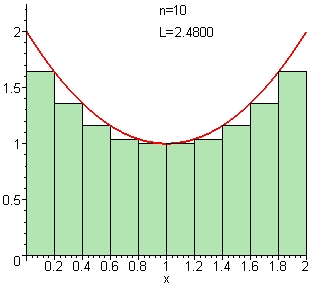
\includegraphics[height=7cm]{./figs/lowersum}
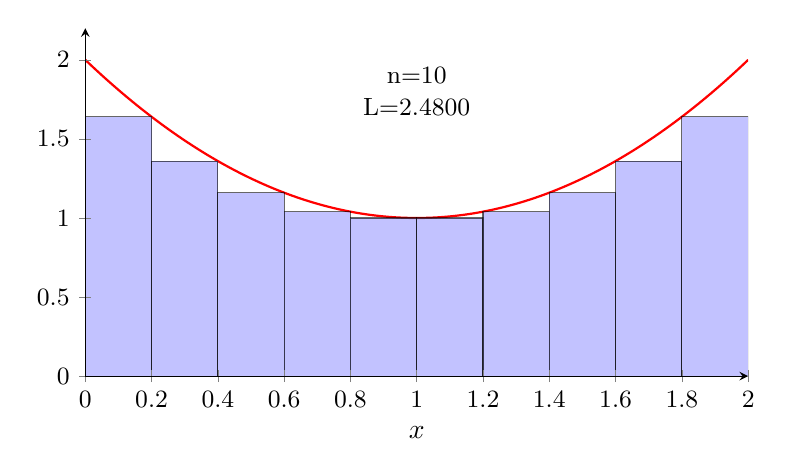
\begin{tikzpicture}
\begin{axis}[
    width=10cm, height=6cm,
    xlabel={$x$}, ylabel={},
    domain=0:2,
    samples=200,
    axis lines=left,
    xtick={0,0.2,...,2},
    ytick={0,0.5,1,1.5,2},
    ticklabel style={font=\small},
    ymin=0, ymax=2.2,
    xmin=0, xmax=2,
    axis on top,
]

% Plot the function
\addplot [
    domain=0:2, 
    red, thick
] {(x - 1)^2 + 1};

% Plot the lower sum rectangles manually
\pgfmathsetmacro{\n}{10}
\pgfmathsetmacro{\dx}{2/\n}
\foreach \i in {0,...,9} {
    \pgfmathsetmacro{\a}{\i * \dx}
    \pgfmathsetmacro{\b}{(\i + 1) * \dx}
    \pgfmathsetmacro{\fa}{(\a - 1)^2 + 1}
    \pgfmathsetmacro{\fb}{(\b - 1)^2 + 1}
    \pgfmathsetmacro{\minf}{min(\fa, \fb)}
    \addplot [
        fill=blue!40!white, draw=black, opacity=0.6
    ] coordinates {
        (\a, 0) (\a, \minf) (\b, \minf) (\b, 0)
    };
}

% Label
\node at (axis cs:1,1.9) {\small n=10};
\node at (axis cs:1,1.7) {\small L=2.4800};

\end{axis}
\end{tikzpicture}

This is a lower bound for $I$
$$
    L < I
$$

\end{center}
\end{frame}
%%%%%%%%%%%%%%%%%%%%%%%%%%%%%%%%%%%%%%%%%%%
\begin{frame}{Graphically: Upper sum}
\begin{center}
  % 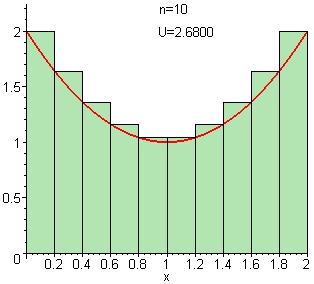
\includegraphics[height=7cm]{./figs/uppersum}
  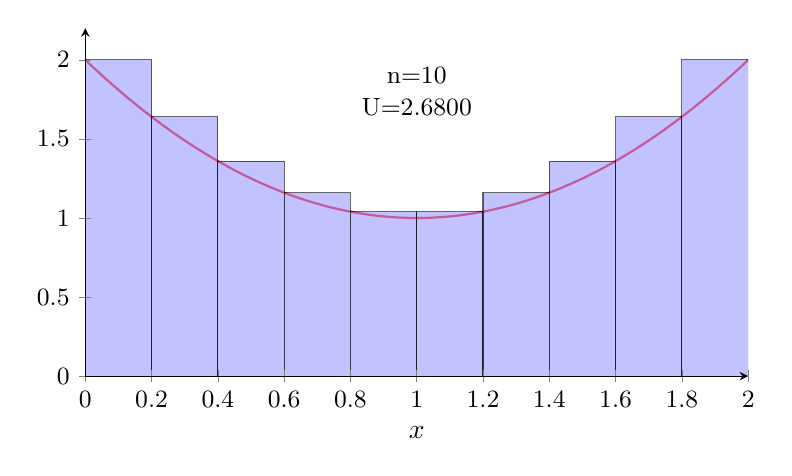
\begin{tikzpicture}
\begin{axis}[
    width=10cm, height=6cm,
    xlabel={$x$}, ylabel={},
    domain=0:2,
    samples=200,
    axis lines=left,
    xtick={0,0.2,...,2},
    ytick={0,0.5,1,1.5,2},
    ticklabel style={font=\small},
    ymin=0, ymax=2.2,
    xmin=0, xmax=2,
    axis on top,
]

% Plot the function
\addplot [
    domain=0:2, 
    red, thick
] {(x - 1)^2 + 1};

% Upper sum rectangles (maximum of endpoints)
\pgfmathsetmacro{\n}{10}
\pgfmathsetmacro{\dx}{2/\n}
\foreach \i in {0,...,9} {
    \pgfmathsetmacro{\a}{\i * \dx}
    \pgfmathsetmacro{\b}{(\i + 1) * \dx}
    \pgfmathsetmacro{\fa}{(\a - 1)^2 + 1}
    \pgfmathsetmacro{\fb}{(\b - 1)^2 + 1}
    \pgfmathsetmacro{\maxf}{max(\fa, \fb)}
    \addplot [
        fill=blue!40!white, draw=black,opacity=0.6
    ] coordinates {
        (\a, 0) (\a, \maxf) (\b, \maxf) (\b, 0)
    };
}

% Labels
\node at (axis cs:1,1.9) {\small n=10};
\node at (axis cs:1,1.7) {\small U=2.6800};

\end{axis}
\end{tikzpicture}

This is a upper bound for $I$
$$
    I<U
$$
\end{center}
\end{frame}
%%%%%%%%%%%%%%%%%%%%%%%%%%%%%%%%%%%%%%%%%%%

\begin{frame}{A Technical Definition}
\begin{itemize}
  \item As $n\to \infty$ the lower and upper sums converge to some number $I$
  $$
    \text{Lower Sum} \le I \le \text{Upper Sum}
  $$

  
\define{The Integral}{
    The integral $\int_a^b f(x) dx$ is the limit 
      $$\lim_{n\rightarrow\infty} L(f;P)$$
    and 
    $$\lim_{n\rightarrow\infty} U(f;P)$$
    when they both agree.
}
\end{itemize}
\end{frame}

%%%%%%%%%%%%%%%%%%%%%%%%%%%%%%%%%%%%%%%%%%%
\begin{frame}{Other Riemann Sums}
There are specific names for sums depending on how we select the sample point 
    $$R(f,P) = \sum_{i=0}^{n-1} f(\underbrace{x^*_i}_{\text{sample point}}) \Delta x_i $$
\begin{itemize}
    \item Upper Sum 
    $$f(x^*_i) = \max_{x\in [x_i, x_{i+1}]} f(x)$$   
    \item Lower Sum
    $$f(x^*_i) = \min_{x\in [x_i, x_{i+1}]} f(x) $$  
    \item $x^*_i = x_i \implies $ \textbf{Left Riemann Sum}
    \item $x^*_i = x_{i+1} \implies $ \textbf{Right Riemann Sum}
    \item $x^*_i = \frac{x_{i+1}+x_{i}}{2} \implies $ \textbf{Midpoint rule}
\end{itemize}
\end{frame}

%%%%%%%%%%%%%%%%%%%%%%%%%%%%%%%%%%%%%%%%%%%
\begin{frame}{Riemann Integration}
\method{Riemann Integration}{Function $f(x)$ continuous on $[a,b]$, partition $P$, way of choosing sample point}{Approximation to $\int_a^b f(x)\,dx$}{Approximate the integral with a finite sum of rectangles.}
\begin{itemize}
    \item The basic Riemann sums are 
    \begin{itemize}
        \item Upper sum
        \item Lower sum
        \item Right Riemann 
        \item Left Riemann 
        \item Midpoint Rule
    \end{itemize}
\end{itemize}
\end{frame}
%%%%%%%%%%%%%%%%%%%%%%%%%%%%%%%%%%%%%%%%%%%
\begin{frame}{Idea of Riemann Integration}
\begin{center}
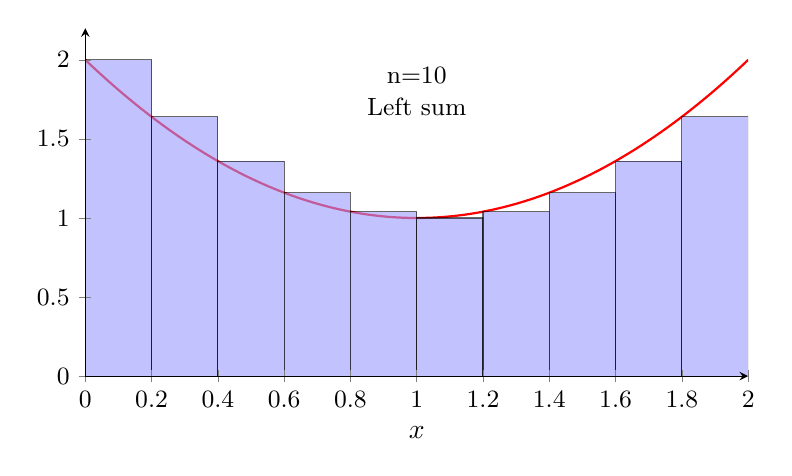
\begin{tikzpicture}
\begin{axis}[
    width=10cm, height=6cm,
    xlabel={$x$}, ylabel={},
    domain=0:2,
    samples=200,
    axis lines=left,
    xtick={0,0.2,...,2},
    ytick={0,0.5,1,1.5,2},
    ticklabel style={font=\small},
    ymin=0, ymax=2.2,
    xmin=0, xmax=2,
    axis on top,
]

% Plot the function
\addplot [
    domain=0:2, 
    red, thick
] {(x - 1)^2 + 1};

% Left-endpoint Riemann sum rectangles
\pgfmathsetmacro{\n}{10}
\pgfmathsetmacro{\dx}{2/\n}
\foreach \i in {0,...,9} {
    \pgfmathsetmacro{\a}{\i * \dx}
    \pgfmathsetmacro{\b}{(\i + 1) * \dx}
    \pgfmathsetmacro{\fa}{(\a - 1)^2 + 1}
    \addplot [
        fill=blue!40!white, draw=black, opacity=0.6
    ] coordinates {
        (\a, 0) (\a, \fa) (\b, \fa) (\b, 0)
    };
}

% Labels
\node at (axis cs:1,1.9) {\small n=10};
\node at (axis cs:1,1.7) {\small Left sum};

\end{axis}
\end{tikzpicture}

\end{center}

\begin{block}{Parameters}
\begin{itemize}
    \item Choose rule: $x_i^*=$ left endpoint
    \item Choose number of rectangles: $n=10$
\end{itemize}
    
\end{block}

\end{frame}

%%%%%%%%%%%%%%%%%%%%%%%%%%%%%%%%%%%%%%%%%%%
\begin{frame}{Overview}
   Understand why some algorithms are better than others. 
   \bigskip
   
   Understand how to evaluate the algorithm performance. 
   \bigskip

   Learn how to implement them. 
   \bigskip

   List of  algorithms:
   \begin{itemize}
     \item Trapezoid Rule
     \item Composite Trapezoid Rule
     \item Simpson's Rule
     \item Composite Simpson's Rule
     \item General Newton-Cotes Rules
   \end{itemize}
\end{frame}
%%%%%%%%%%%%%%%%%%%%%%%%%%%%%%%%%%%%%%%%%%%
\sectionframe{Trapezoidal Rule}
%%%%%%%%%%%%%%%%%%%%%%%%%%%%%%%%%%%%%%%%%%%

\begin{frame}[shrink]{One Shape}
\begin{block}{Integral $\approx$ One Area}
    Suppose you want to approximate an integral with one shape
        $$
            \int_a^b f(x)\,dx \approx \text{area of a shape}
        $$
\end{block}

\begin{figure}
    \centering
    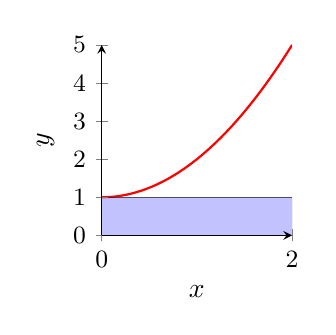
\begin{tikzpicture}
\begin{axis}[
    width=4cm, height=4cm,
    xlabel={$x$}, ylabel={$y$},
    domain=0:2,
    samples=200,
    axis lines=left,
    xtick={0,2},
    ytick={0,1,2,3,4,5},
    ticklabel style={font=\small},
    ymin=0, ymax=5,
    xmin=0, xmax=2,
    axis on top,
]
% Plot f(x) = x^2 + 1
\addplot [
    red, thick
] {x^2 + 1};

% One rectangle (left endpoint at x=0)
\addplot [
    fill=blue!40!white, draw=black, opacity=0.6
] coordinates {
    (0,0) (0,1) (2,1) (2,0)
};
\end{axis}
\end{tikzpicture}
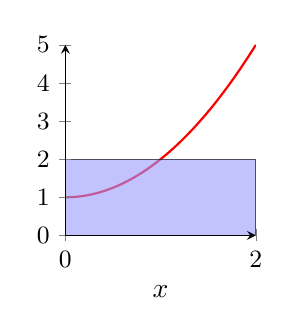
\begin{tikzpicture}
\begin{axis}[
    width=4cm, height=4cm,
    xlabel={$x$}, ylabel={},
    domain=0:2,
    samples=200,
    axis lines=left,
    xtick={0,2},
    ytick={0,1,2,3,4,5},
    ticklabel style={font=\small},
    ymin=0, ymax=5,
    xmin=0, xmax=2,
    axis on top,
]

% Plot f(x) = x^2 + 1
\addplot [
    red, thick
] {x^2 + 1};
% One rectangle (left endpoint at x=0)
\addplot [
    fill=blue!40!white, draw=black, opacity=0.6
] coordinates {
    (0,0) (0,2) (2,2) (2,0)
};
\end{axis}
\end{tikzpicture}
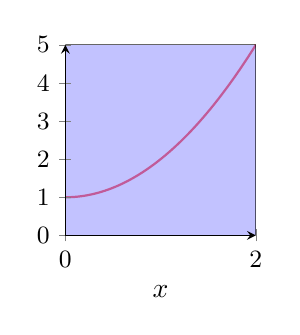
\begin{tikzpicture}
\begin{axis}[
    width=4cm, height=4cm,
    xlabel={$x$}, ylabel={},
    domain=0:2,
    samples=200,
    axis lines=left,
    xtick={0,2},
    ytick={0,1,2,3,4,5},
    ticklabel style={font=\small},
    ymin=0, ymax=5,
    xmin=0, xmax=2,
    axis on top,
]

% Plot f(x) = x^2 + 1
\addplot [
    red, thick
] {x^2 + 1};

% One rectangle (left endpoint at x=0)
\addplot [
    fill=blue!40!white, draw=black, opacity=0.6
] coordinates {
    (0,0) (0,5) (2,5) (2,0)
};
\end{axis}
\end{tikzpicture}

\end{figure}

\end{frame}

% -------------

\begin{frame}{Improvement over Rectangles}
\question{What shape could approximate this area better than this rectangle?}
\begin{figure}
    \centering
    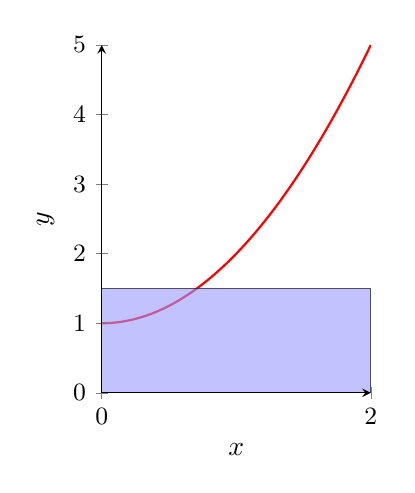
\begin{tikzpicture}
\begin{axis}[
    width=5cm, height=6cm,
    xlabel={$x$}, ylabel={$y$},
    domain=0:2,
    samples=200,
    axis lines=left,
    xtick={0,2},
    ytick={0,1,2,3,4,5},
    ticklabel style={font=\small},
    ymin=0, ymax=5,
    xmin=0, xmax=2,
    axis on top,
]
% Plot f(x) = x^2 + 1
\addplot [
    red, thick
] {x^2 + 1};
% One rectangle (left endpoint at x=0)
\addplot [
    fill=blue!40!white, draw=black, opacity=0.6
] coordinates {
    (0,0) (0,1.5) (2,1.5) (2,0)
};
\end{axis}
\end{tikzpicture}
\onslide<2>{
    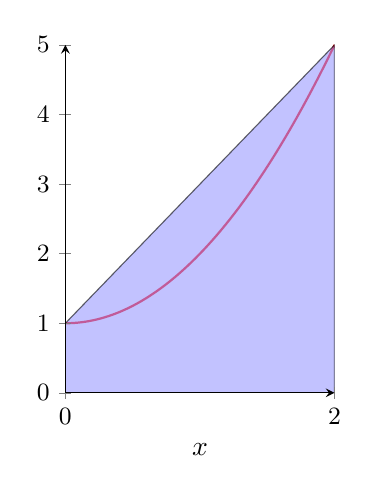
\begin{tikzpicture}
\begin{axis}[
    width=5cm, height=6cm,
    xlabel={$x$}, ylabel={},
    domain=0:2,
    samples=200,
    axis lines=left,
    xtick={0,2},
    ytick={0,1,2,3,4,5},
    ticklabel style={font=\small},
    ymin=0, ymax=5,
    xmin=0, xmax=2,
    axis on top,
]

% Plot f(x) = x^2 + 1
\addplot [
    red, thick
] {x^2 + 1};

% One rectangle (left endpoint at x=0)
\addplot [
    fill=blue!40!white, draw=black, opacity=0.6
] coordinates {
    (0,0) (0,1) (2,5) (2,0)
};
\end{axis}
\end{tikzpicture}
}
\end{figure}
\onslide<2>{
\begin{center}    
A trapezoid
\end{center}
}

\end{frame}

%%%%%%%%%%%%%%%%%%%%%%%%%%%%%%%%%%%%%%%%%%%


\begin{frame}{Trapezoids $>$ Rectangles}
Goal:  Approximate
\begin{equation*}
\int_a^b f(x)\,dx
\end{equation*}
Geometrically, the definite integral is related to the area under $f(x)$.\bigskip
\begin{itemize}
\item Simple Idea: Riemann integration says:\\
   Approximate the area under $f(x)$ with a sum of areas of \underline{rectangles}. 
   \bigskip
\item Better Idea: Trapezoidal rule says: \\ 
Approximate the area under $f(x)$ with a sum of areas of \underline{trapezoids}. \bigskip
\end{itemize}

\keyidea{The area of a trapezoid will better approximate an integral than most rectangles.}
\end{frame}

%%%%%%%%%%%%%%%%%%%%%%%%%%%%%%%%%%%%%%%%%%%%%%%%%%%%

\begin{frame}{Area of a Trapezoid}
\begin{center}
    
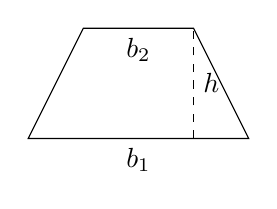
\begin{tikzpicture}[scale = 0.7]
% Define coordinates
\coordinate (A) at (0,0);
\coordinate (B) at (4,0);
\coordinate (C) at (3,2);
\coordinate (D) at (1,2);

% Draw trapezoid
\draw (A) -- (B) -- (C) -- (D) -- cycle;

% Add height label
\draw[dashed] (3,0) -- (3,2);
\node[right] at (3,1) {$h$};

% Add base labels
\node[below] at (2,0) {$b_1$};
\node[below] at (2,2) {$b_2$};
\end{tikzpicture}
\hspace{2cm}
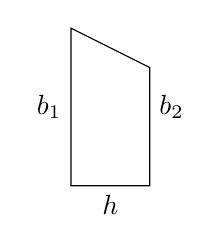
\begin{tikzpicture}[scale=0.5]
% Define coordinates
\coordinate (A) at (0,0);
\coordinate (B) at (2,0);
\coordinate (C) at (2,3);
\coordinate (D) at (0,4);

% Draw trapezoid
\draw (A) -- (B) -- (C) -- (D) -- cycle;

% Add height label
\node[below] at (1,0) {$h$};

% Add base labels
\node[left] at (0,2) {$b_1$};
\node[right] at (2,2) {$b_2$};
\end{tikzpicture}
\end{center}
\begin{itemize}
\item These are both trapezoids
\item The upright trapezoid is the one we care about
\end{itemize}
\begin{block}{Area Formula}
$$A = \frac{b_1+b_2}{2}h$$
    
\end{block}

\end{frame}
%%%%%%%%%%%%%%%%%%%%%%%%%%%%%%%%%%%%%%%%%%%

\begin{frame}{Basic Trapezoid}
\begin{block}{Formula for the Basic Trapezoid Rule}
\begin{equation*}
  \int_a^b f(x) \,dx \approx \frac{f(a)+f(b)}{2}(b-a)
\end{equation*}
\end{block}
\begin{center}
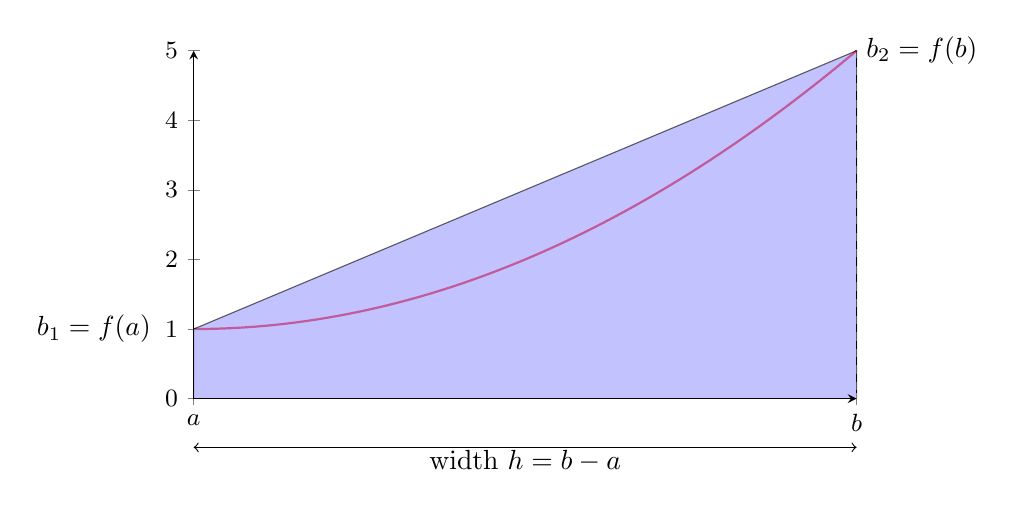
\begin{tikzpicture}
\begin{axis}[
    width=10cm, height=6cm,
    xlabel={}, ylabel={},
    domain=0:2,
    samples=200,
    axis lines=left,
    xtick={0,2},
    xticklabels={$a$,$b$},
    ytick={0,1,2,3,4,5},
    ticklabel style={font=\small},
    ymin=0, ymax=5,
    xmin=0, xmax=2,
    axis on top,
    clip=false
]

% Plot f(x) = x^2 + 1
\addplot [red, thick] {x^2 + 1};

% Trapezoid
\addplot [
    fill=blue!40!white, draw=black, opacity=0.6
] coordinates {
    (0,0) (0,1) (2,5) (2,0)
};

% Vertical dashed lines
\draw[dashed] (axis cs:0,0) -- (axis cs:0,1);
\draw[dashed] (axis cs:2,0) -- (axis cs:2,5);

% Labels for function values
\node[left] at (-0.1,1) {$b_1=f(a)$};
\node[right] at (2,5) {$b_2=f(b)$};

% Width label
\draw[<->] (axis cs:0,-0.7) -- (axis cs:2,-0.7);
\node at (axis cs:1,-0.9) {width $h=b-a$};

% Average height label
% \node at (axis cs:1,3.2) {\small avg height};
% \node at (axis cs:1,2.8) {$\frac{f(a)+f(b)}{2}$};

\end{axis}
\end{tikzpicture}
\end{center}
\end{frame}
%%%%%%%%%%%%%%%%%%%%%%%%%%%%%%%%%%%%%%%%%%%
\begin{frame}{Example}
\begin{example}
Approximate the integral
\[I=\int_{1}^{2} (x^2+1)\,dx \]
using the basic trapezoidal rule.
\end{example}
\begin{itemize}
\item The formula is 
$$
  \int_a^b f(x) \,dx \approx \frac{f(a)+f(b)}{2}(b-a),
$$
where $a=1$, $b=2$, and $f(x)=x^2+1$

\item We get
\[\int_{1}^{2} (x^2+1)\,dx \approx  \frac{(2^2+1)+(1^2+1)}{2}(2-1)=\frac{5+2}{2}=3.5\]
\end{itemize}
\end{frame}
%%%%%%%%%%%%%%%%%%%%%%%%%%%%%%%%%%%%%%%%%%%

\begin{frame}{Example Visualization}

\begin{center}
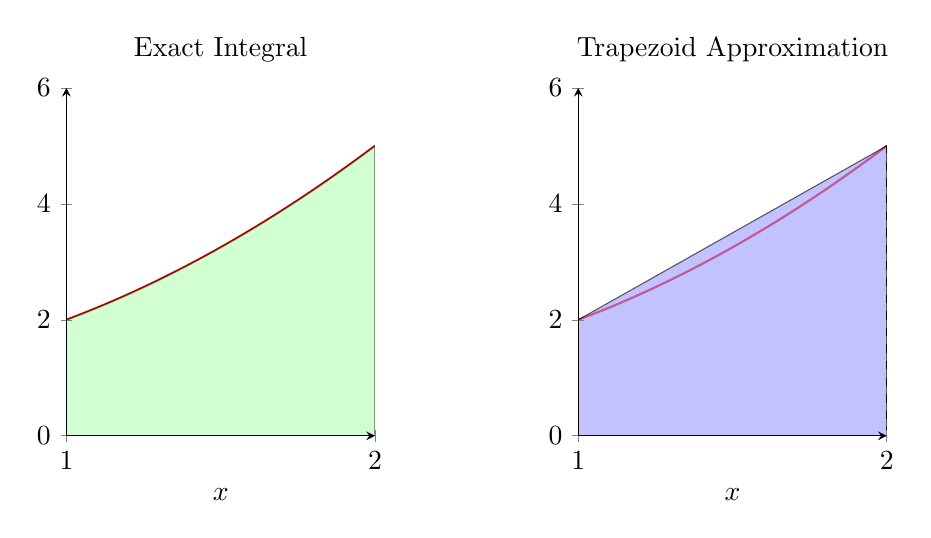
\begin{tikzpicture}
\begin{axis}[
    width=5.5cm, height=6cm,
    at={(0,0)},
    xlabel={$x$},
    domain=1:2,
    samples=200,
    axis lines=left,
    xtick={1,2},
    xticklabels={$1$,$2$},
    ytick={0,2,4,6},
    ymin=0, ymax=6,
    xmin=1, xmax=2,
    title={Exact Integral},
    axis on top
]

% True function
\addplot [red, thick] {x^2 + 1};

% Area under curve
\addplot [
    domain=1:2,
    fill=green!30,
    opacity=0.6
] {x^2 + 1} \closedcycle;

\end{axis}

% ---------------- RIGHT FIGURE ----------------
\begin{axis}[
    width=5.5cm, height=6cm,
    at={(6.5cm,0)},
    xlabel={$x$},
    domain=1:2,
    samples=200,
    axis lines=left,
    xtick={1,2},
    xticklabels={$1$,$2$},
    ytick={0,2,4,6},
    ymin=0, ymax=6,
    xmin=1, xmax=2,
    title={Trapezoid Approximation},
    axis on top
]

% Function
\addplot [red, thick] {x^2 + 1};

% Trapezoid
\addplot [
    fill=blue!40,
    opacity=0.6
] coordinates {
    (1,0) (1,2) (2,5) (2,0)
};

\draw[dashed] (axis cs:1,0) -- (axis cs:1,2);
\draw[dashed] (axis cs:2,0) -- (axis cs:2,5);

\end{axis}

\end{tikzpicture}
\end{center}

\begin{itemize}
\item Left: $I = \frac{10}{3}\approx 3.3333$
\item Right: $I\approx \frac{7}{2}=3.5$
\end{itemize}

\end{frame}

%%%%%%%%%%%%%%%%%%%%%%%%%%%%%%%%
\begin{frame}{One Trapezoid is Not Enough}

\begin{center}
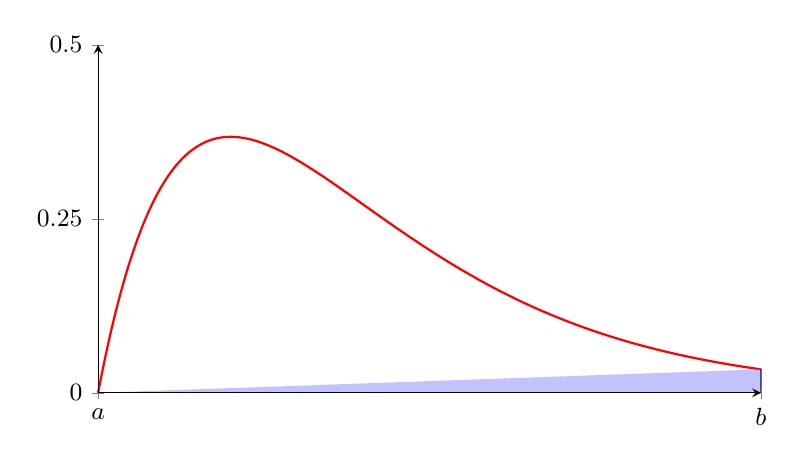
\begin{tikzpicture}
\begin{axis}[
    width=10cm, height=6cm,
    domain=0:5,
    samples=200,
    axis lines=left,
    xtick={0,5},
    xticklabels={$a$,$b$},
    ytick={0,0.25,0.5},
    ticklabel style={font=\small},
    ymin=0, ymax=0.5,
    xmin=0, xmax=5,
    axis on top,
    clip=false
]

% Plot f(x) = x^2 + 1
\addplot [red, thick] {x*exp(-x)};

% Trapezoid
\addplot [
    fill=blue!40!white, draw=black, opacity=0.6
] coordinates {
    (0,0) (5,0) (5,{5*exp(-5)}) 
};
\end{axis}
\end{tikzpicture}
\end{center}

\question{
 How do you resolve this issue?
}


\end{frame}
%%%%%%%%%%%%%%%%%%%%%%%%%%%%%%%%%%%%%%%%%%%%
\begin{frame}{Use Multiple Trapezoids}

\begin{center}
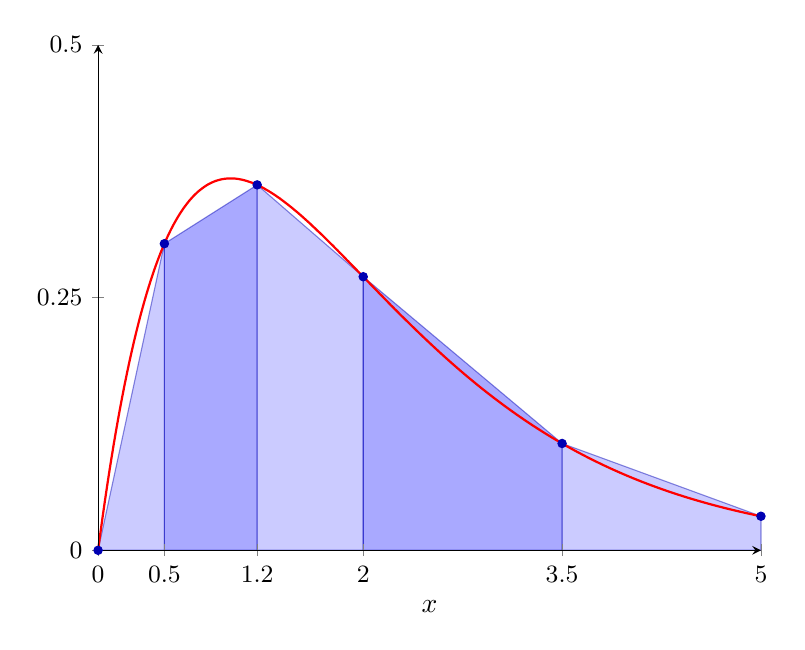
\begin{tikzpicture}
\begin{axis}[
    width=10cm,
    height=8cm,
    axis lines=left,
    xmin=0, xmax=5,
    ymin=0, ymax=0.5,
    domain=0:5,
    samples=300,
    xtick={0,0.5,1.2,2,3.5,5},
    ytick={0,0.25,0.5},
    tick label style={font=\small},
    xlabel={$x$},
    ylabel={},
    axis on top,
    clip=false
]

% Composite trapezoids with nonuniform widths
\addplot[draw=blue!70!black, fill=blue!45, opacity=0.45]
coordinates {
    (0,0) (0.5,{0.5*exp(-0.5)}) (0.5,0)
} \closedcycle;

\addplot[draw=blue!70!black, fill=blue!75, opacity=0.45]
coordinates {
    (0.5,0) (0.5,{0.5*exp(-0.5)})
    (1.2,{1.2*exp(-1.2)}) (1.2,0)
} \closedcycle;

\addplot[draw=blue!70!black, fill=blue!45, opacity=0.45]
coordinates {
    (1.2,0) (1.2,{1.2*exp(-1.2)})
    (2,{2*exp(-2)}) (2,0)
} \closedcycle;

\addplot[draw=blue!70!black, fill=blue!75, opacity=0.45]
coordinates {
    (2,0) (2,{2*exp(-2)})
    (3.5,{3.5*exp(-3.5)}) (3.5,0)
} \closedcycle;

\addplot[draw=blue!70!black, fill=blue!45, opacity=0.45]
coordinates {
    (3.5,0) (3.5,{3.5*exp(-3.5)})
    (5,{5*exp(-5)}) (5,0)
} \closedcycle;

% Exact curve, drawn over the shaded regions
\addplot[red, thick] {x*exp(-x)};

% Nodes on the curve
\addplot[
    only marks,
    mark=*,
    mark size=1.5pt,
    blue!70!black
] coordinates {
    (0,0)
    (0.5,{0.5*exp(-0.5)})
    (1.2,{1.2*exp(-1.2)})
    (2,{2*exp(-2)})
    (3.5,{3.5*exp(-3.5)})
    (5,{5*exp(-5)})
};

\end{axis}
\end{tikzpicture}

Add up multiple trapezoids!
\end{center}
    
\end{frame}

%%%%%%%%%%%%%%%%%%%%%%%%%%%%%%%%%%%%%%%%%%%
\begin{frame}{General Composite Trapezoid}
   \begin{enumerate}
      \item Consider a partition $P=\{x_0=a, x_1, x_2, \dots, x_n = b\}$ of $[a,b]$.

      \item In each interval $[x_i,x_{i+1}]$ of width $h_i$, use the basic Trapezoid:
            \begin{equation*}
              \int_a^b f(x)\,dx \approx \sum_{i=0}^{n-1}
            \frac{f(x_i)+f(x_{i+1})}{2} h_i 
            \end{equation*}
        \item \textbf{Composite Trapezoid} adds the area of $n$ trapezoids
   \end{enumerate}
   
   \begin{center}
    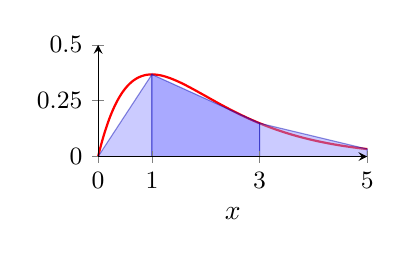
\begin{tikzpicture}
\begin{axis}[
    width=5cm,
    height=3cm,
    axis lines=left,
    xmin=0, xmax=5,
    ymin=0, ymax=0.5,
    domain=0:5,
    samples=300,
    xtick={0,1,3,5},
    ytick={0,0.25,...,0.5},
    tick label style={font=\small},
    xlabel={$x$},
    ylabel={},
    axis on top,
    clip=false
]

% exact curve
\addplot[red, thick] {x*exp(-x)};

% composite trapezoids, h = 1
\addplot[draw=blue!70!black, fill=blue!45, opacity=0.45]
coordinates {(0,0) (0,{0*exp(0)}) (1,{1*exp(-1)}) (1,0)};

\addplot[draw=blue!70!black, fill=blue!75, opacity=0.45]
coordinates {(1,0) (1,{1*exp(-1)}) (3,{3*exp(-3)}) (3,0)};

\addplot[draw=blue!70!black, fill=blue!45, opacity=0.45]
coordinates {(3,0) (3,{3*exp(-3)}) (5,{5*exp(-5)}) (5,0)};
\end{axis}
\end{tikzpicture}\\
The trapezoids do not have to have equal width.
\end{center}
\end{frame}

\begin{frame}[fragile]{Implementation}

\begin{itemize}
    
    \item Need the function 
    $$f(x)$$
    \item Need a vector for the partition 
    $$P=\{x_0=a, x_1, x_2, \dots, x_n = b\}$$
    
    \item Add up the sum in a for loop
\end{itemize}
\begin{lstlisting}[mathescape]
$sum = 0$
for $i=0$ to $n-1$
  $h_i = x_{i+1} - x_i$ % width of this interval
  $sum = sum + h_i \cdot (f(x_i)+f(x_{i+1}))/2$
end
\end{lstlisting}
\end{frame}

%%%%%%%%%%%%%%%%%%%%%%%%%%%%%%%%%%%%%%%%%%%
\begin{frame}{Hand Calculation}


\begin{example}
Approximate the integral

$$
\int_{0}^{4} \sqrt{x}\,dx
$$
using composite trapezoidal method with the partition $P=\{0,2,4\}$.
\end{example}
\begin{align*}
    \int_{0}^{4} \sqrt{x}\,dx &\approx T_1 + T_2\\ 
                               &= h\frac{b_1+b_2}{2} + h\frac{b_2+b_3}{2}\\
                               &= (2)\frac{f(0)+f(2)}{2} + (2)\frac{f(2)+f(4)}{2}\\
                               &= \sqrt0+\sqrt2 + \sqrt2+\sqrt4\\
                               &= 2\sqrt2 +2\approx 4.83\\
\end{align*}



\end{frame}

%%%%%%%%%%%%%%%%%%%%%%%%%%%%%%%%%%%%%%%%%%%
\sectionframe{Uniform Width}
%%%%%%%%%%%%%%%%%%%%%%%%%%%%%%%%%%%%%%%%%%%

%%%%%%%%%%%%%%%%%%%%%%%%%%%%%%%%%%%%%%%%%%%%
\begin{frame}{What's the advantage?}

\question{Is there an advantage to forcing uniform width?}

\begin{center}
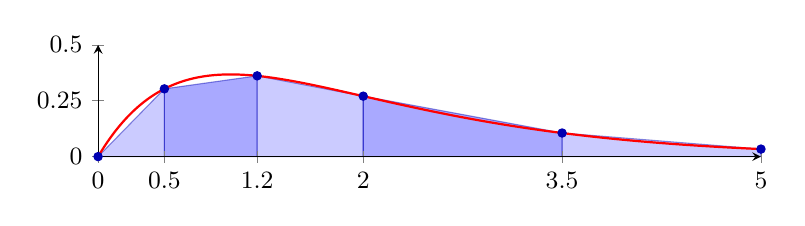
\begin{tikzpicture}
\begin{axis}[
    width=10cm,
    height=3cm,
    axis lines=left,
    xmin=0, xmax=5,
    ymin=0, ymax=0.5,
    domain=0:5,
    samples=300,
    xtick={0,0.5,1.2,2,3.5,5},
    ytick={0,0.25,0.5},
    tick label style={font=\small},
    xlabel={},
    ylabel={},
    axis on top,
    clip=false
]

% Composite trapezoids with nonuniform widths
\addplot[draw=blue!70!black, fill=blue!45, opacity=0.45]
coordinates {
    (0,0) (0.5,{0.5*exp(-0.5)}) (0.5,0)
} \closedcycle;

\addplot[draw=blue!70!black, fill=blue!75, opacity=0.45]
coordinates {
    (0.5,0) (0.5,{0.5*exp(-0.5)})
    (1.2,{1.2*exp(-1.2)}) (1.2,0)
} \closedcycle;

\addplot[draw=blue!70!black, fill=blue!45, opacity=0.45]
coordinates {
    (1.2,0) (1.2,{1.2*exp(-1.2)})
    (2,{2*exp(-2)}) (2,0)
} \closedcycle;

\addplot[draw=blue!70!black, fill=blue!75, opacity=0.45]
coordinates {
    (2,0) (2,{2*exp(-2)})
    (3.5,{3.5*exp(-3.5)}) (3.5,0)
} \closedcycle;

\addplot[draw=blue!70!black, fill=blue!45, opacity=0.45]
coordinates {
    (3.5,0) (3.5,{3.5*exp(-3.5)})
    (5,{5*exp(-5)}) (5,0)
} \closedcycle;

% Exact curve, drawn over the shaded regions
\addplot[red, thick] {x*exp(-x)};

% Nodes on the curve
\addplot[
    only marks,
    mark=*,
    mark size=1.5pt,
    blue!70!black
] coordinates {
    (0,0)
    (0.5,{0.5*exp(-0.5)})
    (1.2,{1.2*exp(-1.2)})
    (2,{2*exp(-2)})
    (3.5,{3.5*exp(-3.5)})
    (5,{5*exp(-5)})
};

\end{axis}
\end{tikzpicture}
    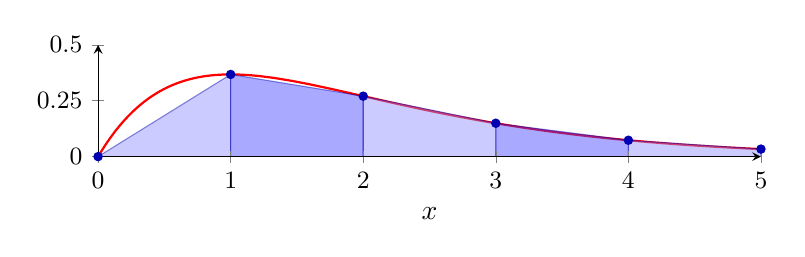
\begin{tikzpicture}
\begin{axis}[
    width=10cm,
    height=3cm,
    axis lines=left,
    xmin=0, xmax=5,
    ymin=0, ymax=0.5,
    domain=0:5,
    samples=300,
    xtick={0,1,...,5},
    ytick={0,0.25,...,0.5},
    tick label style={font=\small},
    xlabel={$x$},
    ylabel={},
    axis on top,
    clip=false
]

% exact curve
\addplot[red, thick] {x*exp(-x)};

% composite trapezoids, h = 1
\addplot[draw=blue!70!black, fill=blue!45, opacity=0.45]
coordinates {(0,0) (0,{0*exp(0)}) (1,{1*exp(-1)}) (1,0)};

\addplot[draw=blue!70!black, fill=blue!75, opacity=0.45]
coordinates {(1,0) (1,{1*exp(-1)}) (2,{2*exp(-2)}) (2,0)};

\addplot[draw=blue!70!black, fill=blue!45, opacity=0.45]
coordinates {(2,0) (2,{2*exp(-2)}) (3,{3*exp(-3)}) (3,0)};

\addplot[draw=blue!70!black, fill=blue!75, opacity=0.45]
coordinates {(3,0) (3,{3*exp(-3)}) (4,{4*exp(-4)}) (4,0)};

\addplot[draw=blue!70!black, fill=blue!45, opacity=0.45]
coordinates {(4,0) (4,{4*exp(-4)}) (5,{5*exp(-5)}) (5,0)};

% nodes on the curve
\addplot[
    only marks,
    mark=*,
    mark size=1.5pt,
    blue!70!black
] coordinates {
    (0,{0*exp(0)})
    (1,{1*exp(-1)})
    (2,{2*exp(-2)})
    (3,{3*exp(-3)})
    (4,{4*exp(-4)})
    (5,{5*exp(-5)})
};
\end{axis}
\end{tikzpicture}\\
\end{center}
    
\end{frame}

% ----------------------
\begin{frame}{Uniform Width}

\begin{block}{General Formula}
$$
\int_a^b f(x)\,dx \approx \sum_{i=0}^{n-1}\frac{f(x_i)+f(x_{i+1})}{2} h_i
$$
\end{block}
If $h$ is uniform...
    \begin{align*}
      \int_a^b f(x)\,dx &\approx \sum_{i=0}^{n-1}\frac{f(x_i)+f(x_{i+1})}{2} h_i\\ 
       &= \sum_{i=0}^{n-1}\frac{f(x_i)+f(x_{i+1})}{2} h\\ 
       &= \frac{h}{2}\sum_{i=0}^{n-1}f(x_i)+f(x_{i+1})\\  
       &= \frac{h}{2}\left(f(x_0) + 2 f(x_1) + 2f(x_2) + \dots + 2 f(x_{n-1}) + f(x_n)\right)
    \end{align*}
\begin{center}
\end{center}
\end{frame}
%%%%%%%%%%%%%%%%%%%%%%%%%%%%%%%%%%%%%%%%%%%
\begin{frame}[fragile]{Compare Formulas}

\begin{block}{General Formula}
$$
\int_a^b f(x)\,dx \approx \sum_{i=0}^{n-1}\frac{f(x_i)+f(x_{i+1})}{2} h_i
$$
\end{block}

\begin{block}{Formula with Uniform Width}
\begin{itemize}
    
  \item The uniform composite trapezoid formula:
\begin{align*}
    \int_a^b f(x)\,dx &\approx \frac{h}{2}\left(f(x_0) + 2 f(x_1) + 2f(x_2) + \dots + 2 f(x_{n-1}) + f(x_n)\right)\\
          &=      h    \left(\frac{1}{2} f(x_0) +   f(x_1) +  f(x_2) + \dots +   f(x_{n-1}) + \frac{1}{2} f(x_n)\right)
\end{align*}
    \item You can save on FLOPs by distributing $\frac12$ 
\end{itemize}
\end{block}
\end{frame}

%%%%%%%%%%%%%%%%%%%%%%%%%%%%%%%%%%%%%%%%%

\begin{frame}[fragile]{Compare Implementation}

\begin{itemize}
\item General 
\begin{lstlisting}[mathescape]
$sum = 0$
for $i=0$ to $n-1$
  $h_i = x_{i+1} - x_i$ % width of this interval
  $sum = sum + h_i \cdot (f(x_i)+f(x_{i+1}))/2$
end
\end{lstlisting}
\item Uniform Width
\begin{lstlisting}[mathescape]
$h = (b-a)/n$
$x = \mathrm{linspace}(a,b,n+1)$
$y = f(x(2:end-1))$ % evaluate f at all interior nodes
$e = (f(a)+f(b))/2$ % endpoints
$I = h \cdot (e+\mathrm{sum}(y))$
\end{lstlisting}
\end{itemize}
    
\end{frame}

%%%%%%%%%%%%%%%%%%%%%%%%%%%%%%%%%%%%%%%%%
\begin{frame}[fragile]{Compare Cost}

\begin{columns}[T]
\begin{column}{0.48\textwidth}
\begin{block}{General Spacing}
For each trapezoid:
\[
    h_i=x_{i+1}-x_i
\]
\[
    S \leftarrow S+h_i\frac{y_i+y_{i+1}}{2}
\]

\begin{itemize}
    \item Width: $1$ FLOP.
    \item Average height: $2$ FLOPs.
    \item Multiply and accumulate: $2$ FLOPs.
\end{itemize}

\[
    \boxed{5n \text{ FLOPs}}
\]
\end{block}
\end{column}

\begin{column}{0.48\textwidth}
\begin{block}{Uniform Spacing}
Compute the width once:
\[
    h=(b-a)/n
\]
Combine heights before scaling:
\[
    S=h\left(\frac{y_0+y_n}{2}
      +\sum_{i=1}^{n-1}y_i\right)
\]

\begin{itemize}
    \item Width: $2$ FLOPs.
    \item Endpoint average: $2$ FLOPs.
    \item Interior additions: $n-1$ FLOPs.
    \item Final scaling: $1$ FLOP.
\end{itemize}

\[
    \boxed{n+4 \text{ FLOPs}}
\]
\end{block}
\end{column}
\end{columns}

\keyidea{
Both cost $O(n)$, but uniform spacing reduces the arithmetic.
Both need only $n+1$ function evaluations if values are stored.
}

\end{frame}
%%%%%%%%%%%%%%%%%%%%%%%%%%%%%%%%%%%%%%%%%%%
\begin{frame}[fragile]{Uniform Composite Trapezoid Formula}

\method{Uniform Composite Trapezoidal Method}{Continuous function $f(x)$, interval $[a,b]$, number of subintervals $n$}{Approximation to $\int_a^b f(x) \,dx$}{Using trapezoids instead of rectangles leads to a better approximation.}

\begin{itemize}
\item Let $h = \frac{b-a}{n}$ and $x_i = a+ih$ for $ i = 0$ to $n$
\item We have an efficient formula 
$$
    \int_a^b f(x)\,dx \approx    h    \left(\frac{1}{2} f(x_0) +   f(x_1) +  f(x_2) + \dots +   f(x_{n-1}) + \frac{1}{2} f(x_n)\right)
$$
\item Constant $h$ simplifies the formula and saves FLOPs
\end{itemize}
\end{frame}


%%%%%%%%%%%%%%%%%%%%%%%%%%%%%%%%%%%%%%%%%%%
\begin{frame}{Example: trap\_int\_test.m}

\begin{itemize}
    \item Test composite trapezoid for
        \begin{equation*}
          \int_0^5 x e^{-x}
        \end{equation*}

    \item The exact solution is known: $\int_0^5 x e^{-x} = 1- 6e^{-5}$

    \begin{alertblock}{}
    What is the order of accuracy?      
    \end{alertblock}
    \bigskip

    \item Find $h^p$ numerically with the test 
        \begin{equation*}
          p \approx \frac{log(err^{(k)}/err^{(k-1)})}{log(h^{(k)}/h^{(k-1)})}
        \end{equation*}
        
    \item Run \texttt{trap\_int\_test.m}
\end{itemize}
\end{frame}

%%%%%%%%%%%%%%%%%%%%
\sectionframe{Summary}
%%%%%%%%%%%%%%%%%%%%

\begin{frame}{Trapezoids are Better than Rectangles}
\begin{center}
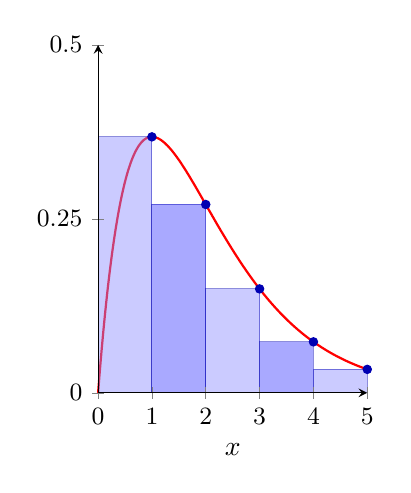
\begin{tikzpicture}
\begin{axis}[
    width=5cm,
    height=6cm,
    axis lines=left,
    xmin=0, xmax=5,
    ymin=0, ymax=0.5,
    domain=0:5,
    samples=300,
    xtick={0,1,...,5},
    ytick={0,0.25,...,0.5},
    tick label style={font=\small},
    xlabel={$x$},
    ylabel={},
    axis on top,
    clip=false
]

% exact curve
\addplot[red, thick] {x*exp(-x)};

% right Riemann rectangles, h = 1
\addplot[draw=blue!70!black, fill=blue!45, opacity=0.45]
coordinates {(0,0) (0,{1*exp(-1)}) (1,{1*exp(-1)}) (1,0)};

\addplot[draw=blue!70!black, fill=blue!75, opacity=0.45]
coordinates {(1,0) (1,{2*exp(-2)}) (2,{2*exp(-2)}) (2,0)};

\addplot[draw=blue!70!black, fill=blue!45, opacity=0.45]
coordinates {(2,0) (2,{3*exp(-3)}) (3,{3*exp(-3)}) (3,0)};

\addplot[draw=blue!70!black, fill=blue!75, opacity=0.45]
coordinates {(3,0) (3,{4*exp(-4)}) (4,{4*exp(-4)}) (4,0)};

\addplot[draw=blue!70!black, fill=blue!45, opacity=0.45]
coordinates {(4,0) (4,{5*exp(-5)}) (5,{5*exp(-5)}) (5,0)};

% right endpoints on the curve
\addplot[
    only marks,
    mark=*,
    mark size=1.5pt,
    blue!70!black
] coordinates {
    (1,{1*exp(-1)})
    (2,{2*exp(-2)})
    (3,{3*exp(-3)})
    (4,{4*exp(-4)})
    (5,{5*exp(-5)})
};

\end{axis}
\end{tikzpicture}
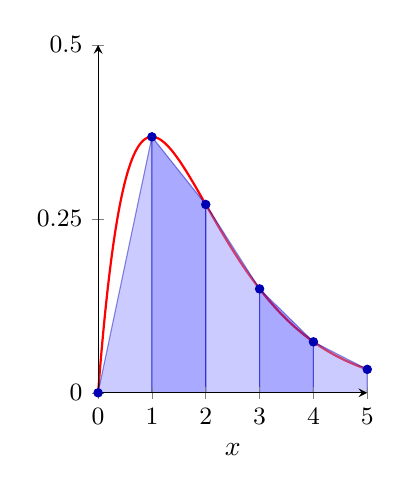
\begin{tikzpicture}
\begin{axis}[
    width=5cm,
    height=6cm,
    axis lines=left,
    xmin=0, xmax=5,
    ymin=0, ymax=0.5,
    domain=0:5,
    samples=300,
    xtick={0,1,...,5},
    ytick={0,0.25,...,0.5},
    tick label style={font=\small},
    xlabel={$x$},
    ylabel={},
    axis on top,
    clip=false
]

% exact curve
\addplot[red, thick] {x*exp(-x)};

% composite trapezoids, h = 1
\addplot[draw=blue!70!black, fill=blue!45, opacity=0.45]
coordinates {(0,0) (0,{0*exp(0)}) (1,{1*exp(-1)}) (1,0)};

\addplot[draw=blue!70!black, fill=blue!75, opacity=0.45]
coordinates {(1,0) (1,{1*exp(-1)}) (2,{2*exp(-2)}) (2,0)};

\addplot[draw=blue!70!black, fill=blue!45, opacity=0.45]
coordinates {(2,0) (2,{2*exp(-2)}) (3,{3*exp(-3)}) (3,0)};

\addplot[draw=blue!70!black, fill=blue!75, opacity=0.45]
coordinates {(3,0) (3,{3*exp(-3)}) (4,{4*exp(-4)}) (4,0)};

\addplot[draw=blue!70!black, fill=blue!45, opacity=0.45]
coordinates {(4,0) (4,{4*exp(-4)}) (5,{5*exp(-5)}) (5,0)};

% nodes on the curve
\addplot[
    only marks,
    mark=*,
    mark size=1.5pt,
    blue!70!black
] coordinates {
    (0,{0*exp(0)})
    (1,{1*exp(-1)})
    (2,{2*exp(-2)})
    (3,{3*exp(-3)})
    (4,{4*exp(-4)})
    (5,{5*exp(-5)})
};

\end{axis}
\end{tikzpicture}
\end{center}
\begin{itemize}
    \item The Riemann sum is a very basic way to approximate integrals 
    \item Adding up trapezoids leads to a better approximation
\end{itemize}
\end{frame}

%%%%%%%%%%%%%%%%%%%%
\begin{frame}{Performance}

\begin{itemize}
    \item The formula is 
    $$
    \int_a^b f(x)\,dx \approx    h    \left(\frac{1}{2} f(x_0) +   f(x_1) +  f(x_2) + \dots +   f(x_{n-1}) + \frac{1}{2} f(x_n)\right)
    $$
    \item The experimental result is 
    $$
        E = \mO(h^2)
    $$

    \item The trapezoid method has \textbf{quadratic accuracy}
\end{itemize}
    
\end{frame}

%%%%%%%%%%%%%%%%%%%%

\begin{frame}{Moving Forward}
\begin{itemize}
    \item Mathematical proof that $E=\mO(h^2)$ (under certain assumptions)
        \vfill 
    \item Simpson's Method - improvement over trapezoid method
        \vfill 
    \item Newton-Cotes methods - a generalization of numerical integration
    \vfill 
\end{itemize}
\end{frame}

\end{document}
